\section{Introduction}\label{introduction}

Technological advances have transformed how museums document, present and interpret their collections, fostering immersive experiences through tools such as laser scanning, 3D printing, and virtual reality \cite{allard2005use,Wachowiak01082009,RCM_2024_3D,Kuzminsky_LaserScan_2012,Schaich_3D_2007}. These technologies place an emphasis on experiential authenticity, enabling encounters that evoke the sensory, emotional, and intellectual essence of the past \cite{trant_Auth_1999}. However, as Pine and Gilmore note \cite{pinegilmore_2007}, achieving authenticity requires museums to navigate the delicate balance between preservation and meaningful engagement—a challenge that is particularly evident in the case of historical musical instrument collections \cite{McAlpine2014}.

Musical instruments represent a distinctive fusion of form, function, and history. Their cultural value extends beyond their visual appeal to include the tactile and auditory dimensions of use \cite{Fritz2017}. Yet, preservation concerns often limit direct interaction, reducing these artefacts to static displays. This ``red velvet cord'' approach, as theorised by McAlpine \cite{McAlpine2014}, protects fragile mechanisms but diminishes the instruments’ functional identity, disconnecting visitors from the full richness of their historical and cultural context.

The Tagliavini Collection in Bologna \cite{Tagliavini2007}, renowned for its historical keyboard instruments, exemplifies this dilemma. To address it, this project introduces an augmented replica of a historical harpsichord keyboard. 
% The project builds on an existing design borrowed from \cite{McPherson2013} and aligns with principles outlined in \cite{Masu_NIME_2023}, emphasising the importance of extending the lifecycle of existing NIMEs. 
The project fosters and complements the augmented piano keyboard design presented by McPherson \cite{McPherson2013} and ensures the relevance of previous NIME designs beyond their original context \cite{Masu_NIME_2023}. 


The article is organised as follows: TBC




% With the advent of digital musical instruments in the 20th century there has
% been a decoupling between interface and sound generation when playing.
% Consequently, aspects of the sensory experience of playing have been lost,
% namely the sensation of vibration and mechanical impedance that a traditional
% musical instrument provides.

% The project aims to restore the tactile and haptic response of historical
% harpsichords for an exhibition at the Museo di San
% Colombano\footnote{https://genusbononiae.it/en/san-colombano-tagliavini-collection/}
% in Bologna. San Colombano is home to the Tagliavini Collection, a collection of
% approximately 70 historical keyboard instruments in working order
% \cite{Tagliavini2007} gifted to the museum by Luigi Ferdinando
% Tagliavini in 2010 \cite{SanColombano2010,Carlino2010}.

% Some items in the Tagliavini collection are no longer in playing condition or
% are too fragile to continue to be available to museum visitors. One of those
% fragile instruments is a 1547 Harpsichord in the Italian style by Alessandro
% Trasuntino \cite{Wraight2024}\footnote{examples of similar instruments by
% Trasuntino available online in the Royal College of Music Collection (1531:
% \url{https://museumcollections.rcm.ac.uk/collection/Details/collect/58}) and the
% Musée de la musique collection (1538:
% \url{https://carmentis.kmkg-mrah.be/eMP/eMuseumPlus?service=ExternalInterface&objectId=106088})
% }, which was used as the basis for an interactive exhibition arranged by San
% Colombano. Part of the exhibit is a keyboard that replicates the mechanism of
% the Trasuntino that aims to provide a similar tactile playing experience to that
% of the original.

% The project was also open-sourced to allow for others to easily recreate and
% iterate on the designs.

% The "Haptic Key" project by Timmermans et al. \cite{Timmermans2020} began with
% the model of a piano key. A 3-key cross-sectional model of a harpsichord
% mechanism \ref{fig:3key} was provided to the NEMUS project by San Colombano as a
% test bed for sensors and as proof of concept for a larger scale interface. Each
% key of the model has 2 sets of strings that are under tension but not at any
% specific musical pitch. The strings are there to provide the same resistance to
% the jack plectra as would be found on an instrument. The mechanism is in the
% Italian style of the XVI-XIX century with 2 jacks per key and their
% corresponding strings tuned in unison \footnote{``8'-8' È la disposizione normale
% dei clavicembali italiani'' \cite{Tagliavini1987}}. 

% A suitable sensing system was found to reliably detect when a jack had plucked a
% string independently and then send a corresponding MIDI message to a connected
% audio engine. A full scale 49-key scale model was commissioned with and then
% built by the luthier \anon{Roberto Livi} in the same style as the 1547 Trasuntino
% \ref{fig:teaser}. The sensor system was installed into the full-scale model and
% then set up for exhibition at San Colombano. Visitors are invited to play on the
% interface, which currently triggers samples on a connected sound engine. The
% paper looks at the design decisions, processes, and considerations that need to
% be made when undertaking a project of this kind.



% Overview of fabrication methods, techniques that can be employed.
% Finally a discussion of the limitations and areas in which the core
% project can be improved and developed further.

% In this context, a `traditional' instrument is one whose interface for
% generating sound and the sound generating mechanism are fundamentally
% coupled. A piano requires a key press which triggers a hammer, which
% strikes a string which vibrates a body and air cavity. This system is
% tied together and cannot be separated. A synthesizer, be it a theremin,
% a control voltage synthesizer, a MIDI controller, these are all
% instruments whose interface are decoupled from their sound generation.
% This decoupling presents a problem that then needs to be addressed. How
% do we re-introduce this dimension to the experience of playing a musical
% instrument? How do we, and is it possible to, parameterise and preserve
% this experience? This is central problem that is trying to be solved in
% \cite{Nichols2002, Timmermans2020, McAlpine2014, Baldwin2016}.

% This is particularly pertinent as it relates to the conservation of musical
% instruments, as they represent both historic objects, but also tools for
% creating music. Historical musical instruments present an interesting
% problem for cultural heritage as they are both a physical object, but
% also a tool for making music. This begs the question, can we use haptics
% to preserve experiences of the past? The proposed project intends to
% develop further the methodologies implemented in musical haptics
% projects \cite{MusicalHaptics2018} such as \cite{Timmermans2020}.

% Systems exist already for the conversion of piano keyboard. The Yamaha
% disklavier, the Don Buchla designed MOOG Piano Bar, Bosendorfer, PNOscan
% by QRS focus on reproduction. These same systems could be applied to a
% harpsichord, but the limitation is a single data stream per key.

% \subsection{Motivations}\label{motivations}


% \begin{itemize}
% \item
%   existing sysetms
%   \begin{itemize}
%   \item
%     Yamaha Disklavier used as a basis for exploration into haptics and
%     the piano keyabord
%     \cite{MusicalHaptics2018_04, MusicalHaptics2018_05,
%     MusicalHaptics2018_13}
%   \item
%     Bosendorfer: LED photo transistor pair \cite{Moog1990} for obtaining
%     performance data \cite{MusicalHaptics2018_05}

%     \begin{itemize}
%     \item
%       290SE
%     \item
%       CEUS
%     \end{itemize}
%   \item
%     Don Buchla / Moog Piano Bar
%   \item
%     PNOscan MIDI 9 QRS Music as MIDI Piano system \cite{McPherson2013}

%     \begin{itemize}
%     \item
%       PNOmation
%     \end{itemize}
%   \item
%     Piano Disc
%   \end{itemize}
% \end{itemize}

\section{Related Work and Motivations}\label{related-work}

% These systems mentioned could be adapted for a harpsichord, but they would not
% easily capture the separate plucks from both jacks per key. We decided to create
% our own system and focus on detecting the vertical displacement of the jacks
% directly, rather than the position of the key.

% Methodologies for increasing visitor engagmemnet or

% Museum staff want visitors to be engaged but limits in staffing and
% funding limit how vistors can interact with collections
% \cite{Templeton2018,
% McAlpine2014}. For musical instrument museums there is an additional
% difficulty in the balance of keeping historical instruments playable
% \cite{McAlpine2014}. The fragility and decay of musical instruments
% means that there is an inveitable point where instruments will no longer
% be in a playable condition \cite{McAlpine2014, Fritz2017}

% McAlpine outlines a similar situation to the Tagliavini collection in
% his work with the Benton Fletcher Collection \cite{McAlpine2014}. There
% was a stipulation by Benton Fletcher that the instruments remain
% available to play when they were gifted to National Trust Fenton House.
% A custom MIDI interface arranged in a two manual harpsichord style which
% triggered samples of the instruments in the collection using an
% appropraite recording strategy for each. One problem highlighted in user
% tests by McAlpine is that the weighted keys did no provide ``an
% experiential sense of interacting with a historical keyboard''
% \cite{McAlpine2014}. The MIDI interface created from commercially
% available weighted keys. McAlpine posits a haptic keyboard augemented
% with ``actuators to provide positionally-sensitive real-time force
% feedback at point-of-contact'' in a similar approach as the piano
% mechanism by Gillespie \cite{Gillespie1996}.

% Previous NIME project ``Tromba Moderna'' \cite{Baldwin2016} looked to
% avoid the complex engineering problem by simply recreating the tromba
% marina and augmenting it. In the case of the Tromba Modern, a piezo
% transducer was connected to a sound synthesis engine connected to a
% driver inside the instrument to simulate the vibration that would be
% expected of an historical tromba marina.

% The original design was to take a similar approach to the project by
% Timmermans \cite{Timmermans2020}, which was an extension of the system
% by Gillespie \cite{Gillespie1996}. The process laid out in Timmermans
% project was to begin with a single key model of the mechanism. We began
% with a 3-key Model Harpsichord Mechanism by Graziano Bandini
% \textbackslash figure\{\}. Before we continued with augementing a model
% with actuators it was decided that it we should first validate whether a
% recreation of the harpsichord mechanism would suffice in allowing
% visitors to suspend disbelief.

% Benefits of putting effort into the maintenance of one interface with a
% transferable sensor system

% An additonal factor not faced in the Tromba Moderna project is the
% problem of scale in managing 98 rather than a single data stream of
% data.

% Material costs mitigated by creating a scaled version of the sound
% board, providing only the length of string necessary under comparable
% tension and thus resistance to the jack quill.

% Finally, a further extension to the projects above was a commmitement to
% open sourcing all aspects of the project, hardware, software, and data.

% There are commercial systems for augmenting piano keyboards generating MIDI data.

% An additional goal of the project was to design an interface that could be used to research
% the influence the mechanism and it's resistances have on a player's performance.
% For example, the Yamaha Disklavier series of pianos have an embedded sensor
% system that allows for the instruments to operate in a "silent mode", but still
% output MIDI data when the keys are struck. This has been a rich avenue for
% exploring the affect of vibration on performance,
% \cite{MusicalHaptics2018_04,MusicalHaptics2018_13} perception in instrument
% quality \cite{MusicalHaptics2018_05}.

% As well as a trying to offer a more engaging experience to museum attendees, the
% interface was also designed as a potential probe for further research into the
% idiosyncrasies of the harpsichord and the influence the mechanism has on
% performance.


Museums often face significant challenges in engaging visitors due to limitations in staffing and funding, which restrict the ways in which visitors can interact with collections \cite{Templeton2018, McAlpine2014}. For musical instrument museums, these challenges are compounded by the difficulty of preserving historical instruments in a playable condition \cite{McAlpine2014}. The instruments' inherent fragility and gradual decay inevitably result in a point where they can no longer be played, even when collections adhere to the strictest conservation protocols. A significant cultural change has taken place in recent decades, shifting the focus from the playability of the originals to their conservation. Karp \cite{Karp1979,Karp1985} advocates for a deeper understanding of musical instruments so that enough knowledge is generated to make them as ``copyable'' as possible.

McAlpine discusses a case similar to the Tagliavini collection in his examination of the Benton Fletcher Collection at National Trust Fenton House \cite{McAlpine2014}. When these instruments were donated, Benton Fletcher stipulated that they remain playable and should continue to be maintained for tuition and public performance. A large sampling campaign was conducted, and a custom MIDI interface was designed to fulfil this requirement while preserving the original instruments' integrity. The MIDI keyboard, comprising two commercially available keyboards mimicking the two-manual harpsichord layout, were used by visitors to trigger the instrument samples recorded with tailored strategies for each. However, user tests identified a significant limitation: the commercially available weighted keys failed to provide an authentic sense of interacting with a historical keyboard \cite{McAlpine2014}. 

% To address this, McAlpine suggested designing a haptic keyboard enhanced with actuators capable of delivering positionally sensitive, real-time force feedback at the point of contact, inspired by previous projects such as Gillespie’s work on piano mechanisms \cite{Gillespie1996}.

On the other hand, the ``Tromba Moderna'' project \cite{Baldwin2016}, a previous NIME initiative, approached the issue of musical heritage playability by recreating and augmenting a replica of a historical tromba marina. A piezo transducer was connected to a sound synthesis engine and a driver within the instrument to simulate the expected vibrations of a historical tromba marina. 

This work inherits the same philosophy as the Tromba Moderna project. By augmenting a replica of a historical harpsichord keyboard using minimally invasive electronics and controlling a MIDI-triggered sample library, the project intends to offer a tool enhancing the fruition of the Tagliavini collection whilst retaining a form of continuity with historical instrument-building traditions. Furthermore, the electronics design borrows ideas from a previous NIME by McPherson \cite{McPherson2013}. As such, the interface proposed here is not, strictly speaking, a \emph{new} musical interface, particularly in its haptic response designed to adhere to longstanding harpsichord building traditions. However, this work complements and follows up on previous reflections regarding the \emph{sustainability of results} within the NIME community and identified as \emph{the O in NIME} \cite{Masu_NIME_2023}. The intended use of the keyboard through meaningful interaction with a museum exhibit is where the novelty of this work lies, rather than solely in its technological development. 

Beyond enhancing the visitor experience, future design iterations will serve as a research tool to explore the unique characteristics of the harpsichord and its impact on performance through the \anon{ERC-funded NEMUS} project, aiming to virtually reproduce the sound of historical keyboard instruments, and upcoming projects such as Rem@ke \cite{remake1}.

\section{Design}\label{design}

The present project initially drew inspiration from Timmermans' extension of Gillespie’s system \cite{Timmermans2020, Gillespie1996}. Timmermans’ process began with a single-key model of the mechanism. Similarly, we started with a 3-key model harpsichord mechanism, crafted by Graziano Bandini. Before incorporating actuators into the model, we sought to validate whether a faithful recreation of the harpsichord mechanism could effectively enable visitors to suspend disbelief.

\begin{figure}  
  \centering
  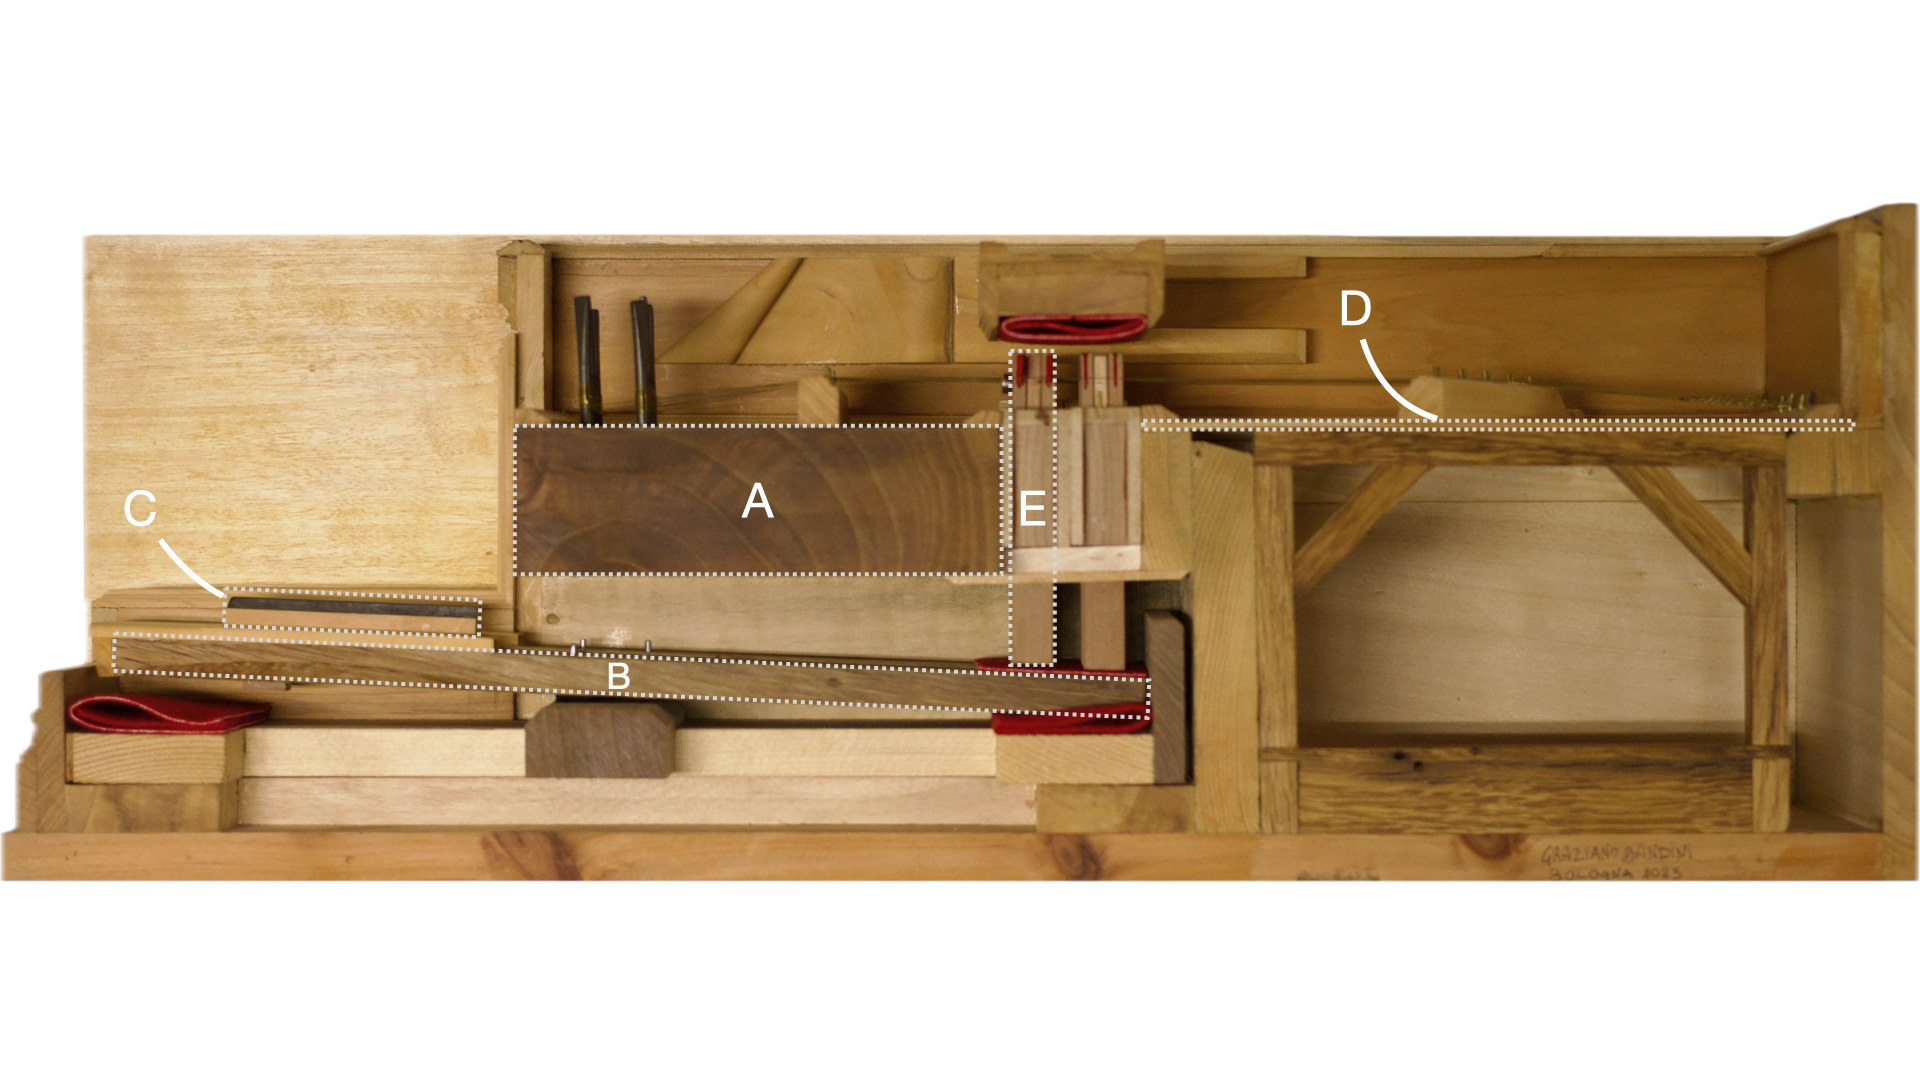
\includegraphics[width=\linewidth]{src/images/3-key-side-labelled.png} 
  \caption{3-key Model Harpsichord Mechanism by Graziano Bandini, Bologna 2023. 3-Key modelled used for initial prototyping. A: Wrestplank B: Key Lever C: Key cap D: soundboard E: Jack} 
  \Description{A 3-Key Model of a Harpsichord Mechanism created Graziano Bandini in Bologna. A side view of the model which is a cross-section of what is a common
mechanism for an Italian style harpsichord of the XVI century.} 
  \label{fig:3key}
\end{figure}

A critical benefit of focusing on the development of a single interface with a transferable sensor system is the potential for scalability and adaptability. However, managing data streams presents a significant challenge. Unlike the Tromba Moderna project, which dealt with a single data stream, our design must manage 98 simultaneous data streams. This complexity necessitated cost-effective solutions, such as scaling down the soundboard to include only the necessary string length under comparable tension and resistance to the jack quill.

Another distinguishing feature of this project is its commitment to open-sourcing all hardware, software, and data components. While commercial systems for augmenting piano keyboards and generating MIDI data exist, this project emphasizes accessibility and transparency.

An additional objective was to design an interface that supports research into how the harpsichord mechanism and its resistances influence a player’s performance. For example, the Yamaha Disklavier series incorporates embedded sensors enabling "silent mode" operation while outputting MIDI data when keys are struck. This has facilitated research into the effects of vibration on performance \cite{MusicalHaptics2018_04, MusicalHaptics2018_13} and the perception of instrument quality \cite{MusicalHaptics2018_05}.

\section{Design}

The design criteria was to create a keyboard interface that provided a comparable tactile response to that of a harpsichord in the italian style.

Accommodations were made in the design to allow for as much flexibility as possible. 
This also meant that designs for the electronics would have to include a level of flexibility in how they might be installed. 
Surplus space was added into the design of the internal chamber of the model Figure \ref{fig:49-key-bottom}, but there was still a limit given the structural
and aesthetic requirements.

\section{Constraints}\label{design-problem}

% Central philosophy of the Tagliavini Collection is that the instrument
% should remain playable to the public. The condition of some instruments
% is such that restoration would required a replacement of vast majority
% of the instrument, would be too costly, would risk the instrument given
% its fragility, or all of those in combination.

% This is not an uncommon problem faced by musical instrument museums
% worldwide. The central question the project tries to answer is ``how do
% we conserve musical instruments in order to continue interacting with
% them''

% The approach taken was to recreate the interface of these instruments
% not for acoustics purposes be purely for the mechanical response. As
% exhibition for the general public in a musical instruments there were
% aesthetic and functional constraints placed on the design of the
% interface.

% \subsection{Design Constraints}\label{design-constraints}

There were constraints that were put in place by the Museum on the design of the exhibit.

\begin{itemize}
\item
  No electronics should be visible \footnote{with the exception of a pair of headphones for listening and a display to change parameters of the audio engine}
\item
  It should be robust and reliable, easily maintained by museum staff without complex technical processes
\item
  it should not augment or fix the mechanics, but present them with their original limitation
\end{itemize}

% Another constraint was that the design of the sensor system and the
% model keyboard would have to carried out at a distance in separate
% workshops. Time constraints meant the keyboard was being fabricated for
% a sensor that did not yet exist.


\subsection{Building the Model Keyboard}\label{keyboard}

% PARAGRAPH FROM ROBERTO
The construction of the keyboard required three months of work to be fully completed
and followed the same construction phases of a real harpsichord.

The model was constructed using the materials of the Italian harpsichord
tradition. Parts are labelled in Figure \ref{fig:3key}.

\begin{itemize}
\item
  Walnut wood for the wrestplank
\item
  Chestnut wood for the key levers
\item
  Boxwood and ebony for the key caps.
\item
  Cypress wood for the soundboard
\item
  Beech wood, a brass spring and a seagull feather plectrum for the 98 jacks
\end{itemize}

The body of the case is based on a rectangular poplar frame that leaves space
for the installation of the electronic sensors.

Deviations from the design of the Trasuntino are the rectangular, rather than
'logarithmic' shape, removal of a bottom panel and omission of a short octave,
instead spanning 4 octaves beginning on C.

The strings are Malcolm Rose yellow brass wire, which are secured to wrought
iron pins. The tension of each string was adjusted to provide resistance to
plucking close to that of a harpsichord. Three felt strips were woven between
the strings in order to dampen the vibration of the strings.

The result is an interface instrument that is placed between the mechanical
action of the keys and the generation of a synthetic sound. The touch of the
wooden keys, the friction of the natural feathers on the string, the noise of
the percussion at the base of the key together produce the sensation of being in
front of a real harpsichord.


% \subsubsection{Anatomy of Harpsichord
% mechanics}\label{anatomy-of-harpsichord-mechanics}

% \begin{itemize}
% \item
%   simple
% \item
%   aesthetics
% \item
%   split workload
% \item
%   parts of harpsichord

%   \begin{itemize}
%   \item
%     jack

%     \begin{itemize}
%     \item
%       quill
%     \item
%       jack body
%     \item
%       pivot
%     \item
%       tongue
%     \end{itemize}
%   \item
%     key
%   \item
%     body
%   \end{itemize}
% \end{itemize}

% The decision was made to design the electronics and the model keyboard simultaneously. 
% This meant development development time was quicker and iteration on the idea.
% Likely the first implementation would need re-designed and redesiginng
% the electronics to fit the form of the keyboard was more cost effective
% than building or carrying out major modifications to the model.

% The model was designed to have two internal chambers a front and rear.
% The front and back that was xxx by yyy by 370mm between the faceplate
% and the jacks. The TONGUE THAT GOES INTO SLOT divides the chamber through
% a small gap between the underside of the soundboard and the key guides.
% The key guide needs to be deep enough to allow for the full movement of
% the key and stop the key becoming unseated. The chamber then extends to
% a support wall which divides the front and rear.

% Discussion of spatial constraints and effects on electronics design and
% installation is covered in \textbackslash section\{setup\}

% The rear chamber was designed to house components for audio processing,
% which is discussed further in \textbackslash section

\begin{figure}  
  \centering
  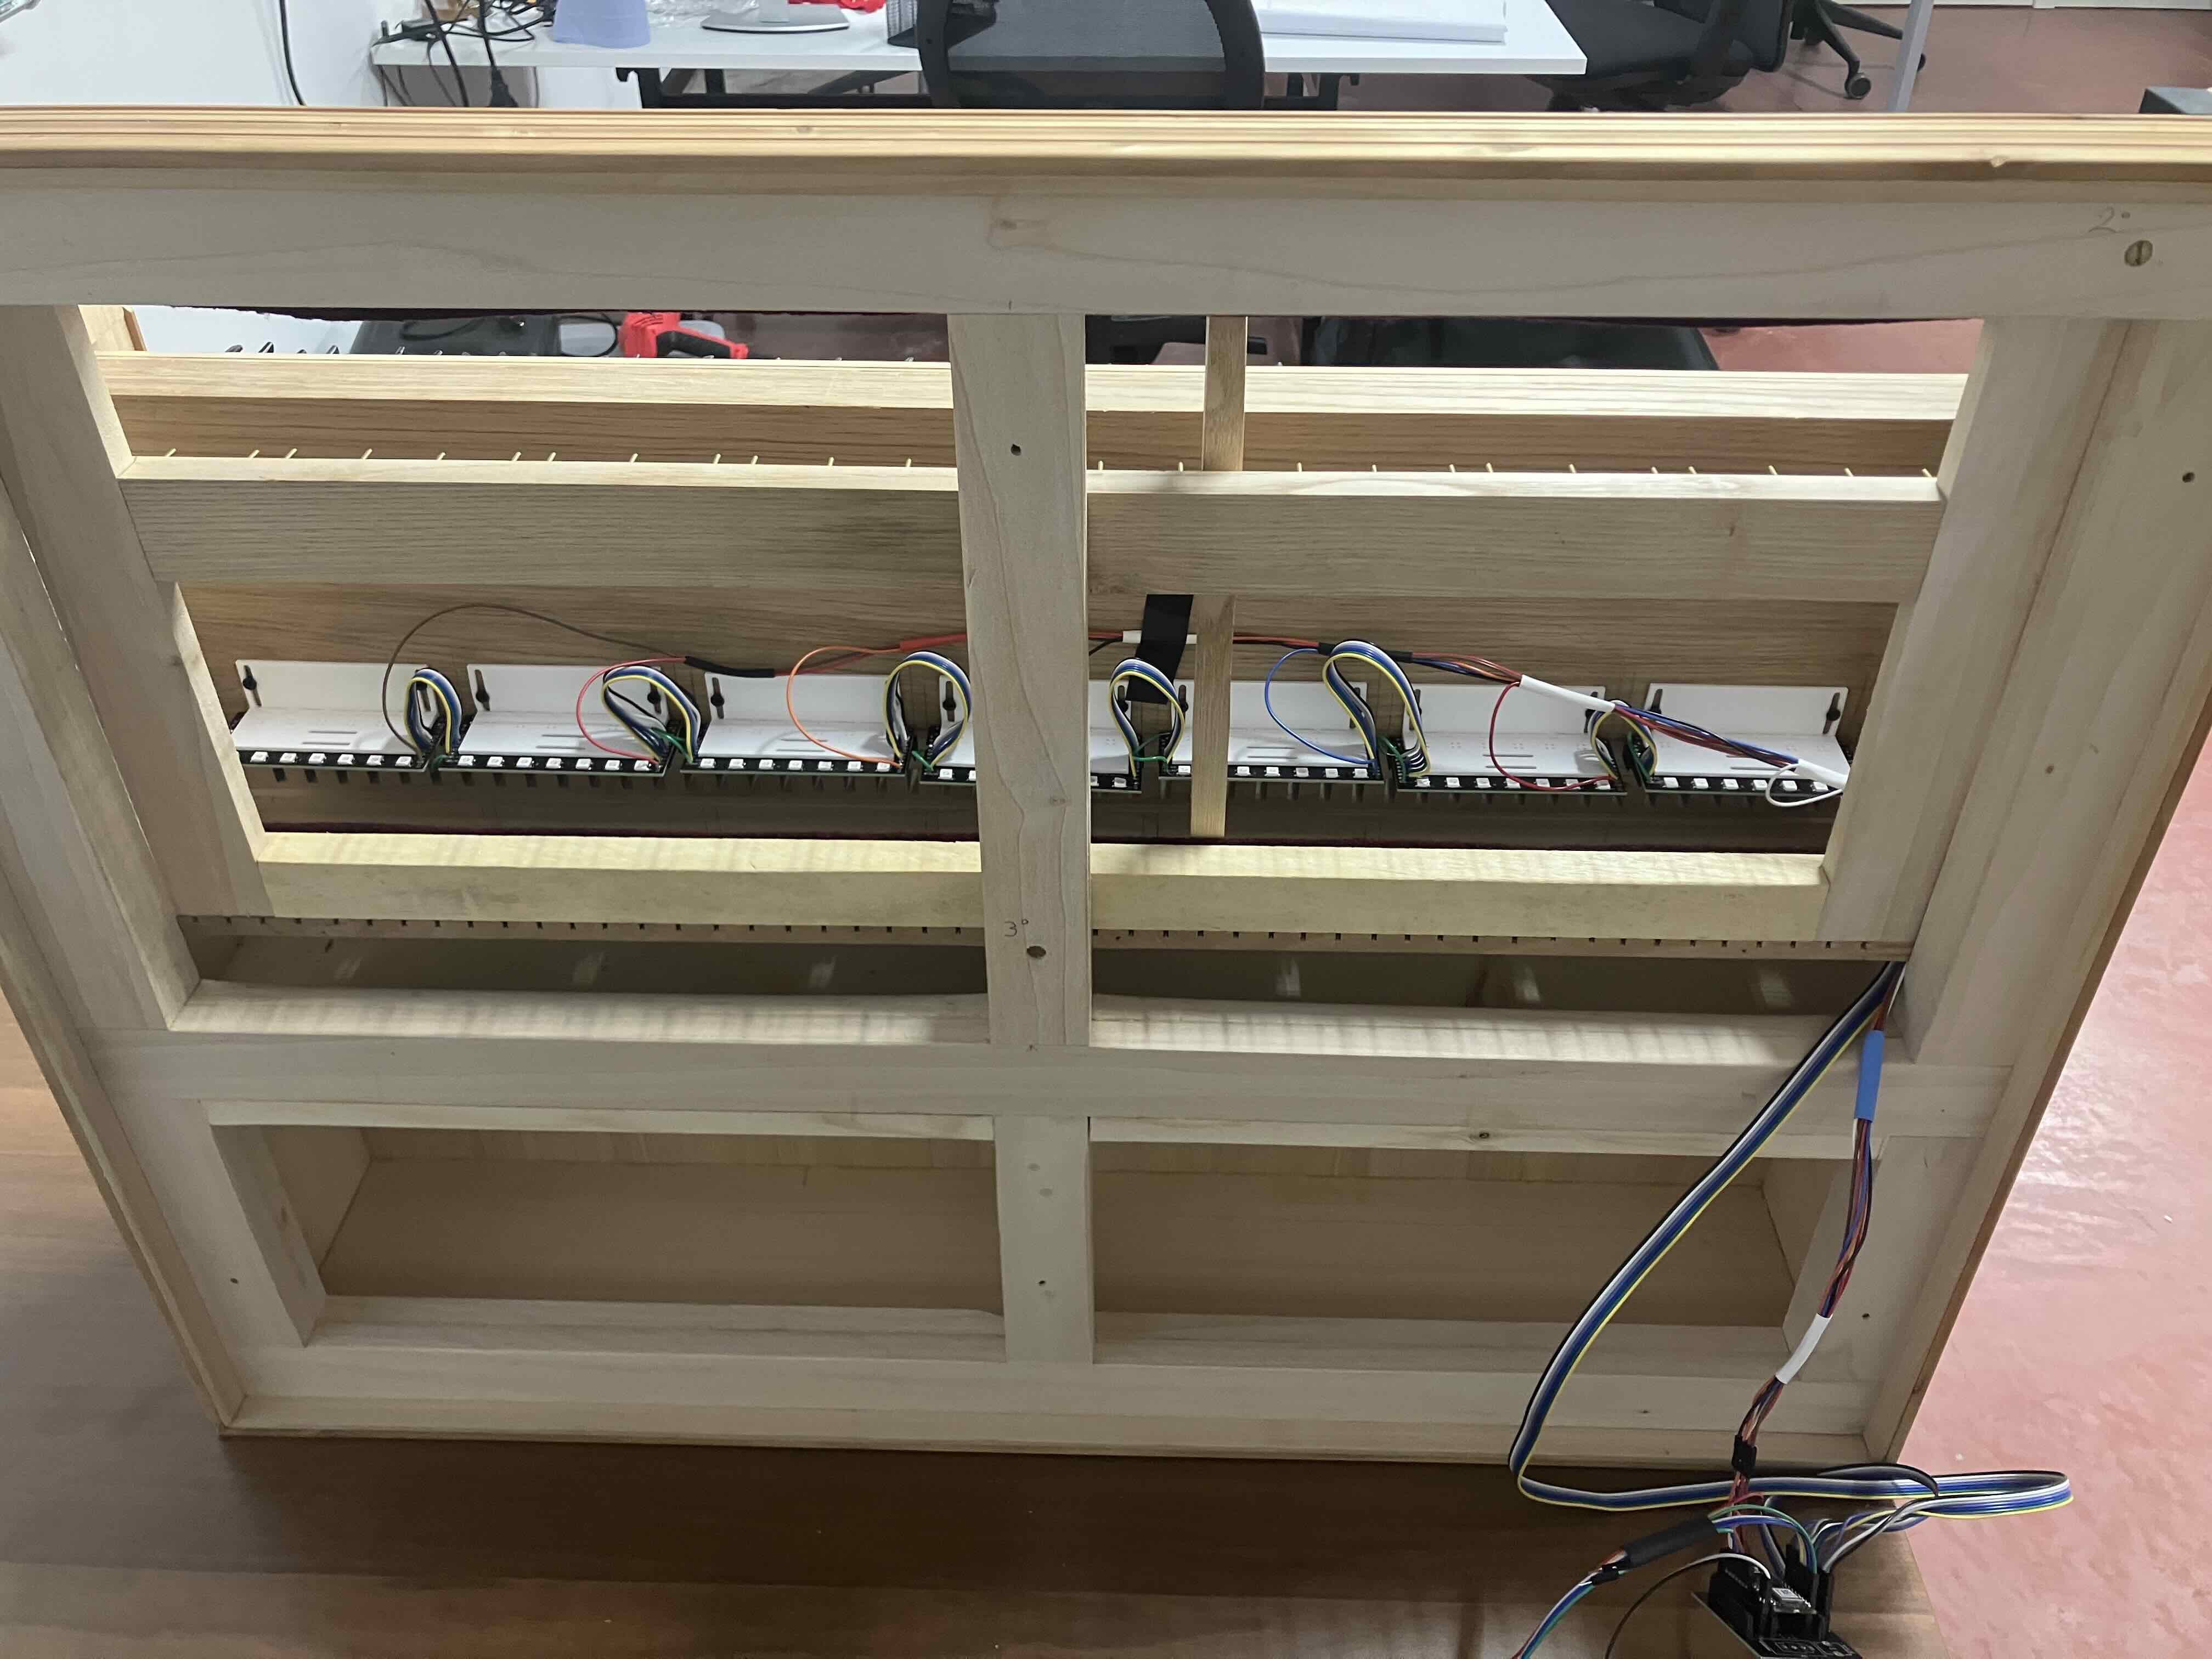
\includegraphics[width=\linewidth]{src/images/49-key-bottom-sensors-no-keys.jpg} 
  \caption{Underside of the full model keyboard showing two chambers. Front chamber at the top and rear chamber at the bottom.} 
  \Description{} 
  \label{fig:49-key-bottom}
\end{figure}

% \footnote{https://github.com/Nemus-Project/haptic-harpsichord-nime-2025/issues/Nemus-Project/haptic-harpsichord-nime-2025/images/disegno.pdf}



% A harpsichord that
% was economic enough to be deconstructed would also have been of a more
% modern mechanical design and not of the design that was being recreated
% with the model. Prototyping stage would likely be invasive and damage or
% heavy modification likely. As such it was not a good use of funds as a
% modern instrument fit for destruction did not offer benefits that the
% small model with easy internal access did not already provide.



% \subsubsection{3-Key Prototype}\label{key-prototype}

% \begin{itemize}
% \item
%   proof of concept
% \item
%   available on loan from museum
% \item
%   easy access to internal structure
% \end{itemize}

% \subsubsection{49-Key Prototype}\label{key-prototype-1}

% For the final interface a 49-key (4-octave) was constructed by luthier
% \anon{Roberto Livi}. The keyboard is in the same style† as the 3-key model with
% to jacks per key.

% The keyboard is fully enclosed and internally has two chambers, front
% and rear, in which the electronics could be installed
% \textbackslash figure(underside 49-key).

% Keyboard to be used for exhibition at san colombano where it would be
% available to play by general public.

% Timescale: from initial discussion to delivery of interface to the \anon{NEMUS}
% lab was 8-months. Active assembly of the instrument was 3 months

% Constructed From:

% \begin{itemize}
% \item
%   for exhibition
% \item
%   problems of scale
% \item
%   problems of timescale
% \end{itemize}

\section{Hardware Design}

For the first iteration the data from the sensor would simply be used to test when a threshold had been passed. On passing the threshold a message would be sent to trigger the playback of a corresponding note.

For the initial prototyping stage, modifying an existing harpsichord was considered though ultimately discarded. An existing instrument would
have provided a test for scaling the electronics, but internal measurements and layout would have been too different. 

Using a similar approach to Timmermans' Haptic Key project, \cite{Timmermans2020} our first step was to fabricate or procure a model of a single working key. San Colombano was able to provide a model 3-key of a harpischord mechanism by Graziano Bandini (Figure \ref{fig:3key}).

\subsection{Sensor Criteria}\label{sensor-criteria}

A set of criteria was drawn to which the final sensor system would have
to satisfy. This criteria was used as a means of evaluating the
feasibility throughout the prototyping phase.

\begin{itemize}
\item
  Non-invasive: The sensor system should not require major modifications
  to the interface on which it is installed.
\item
  Low Latency: Reading sensors and then triggering an output should have
  a low latency. Following \cite{Jack2016} an latency was set as 10 ms
  with an upper limit set to 25ms beyond which the sensors would be
  deemed unusable
\item
  Reliable: Data obtained should be reliable and accurate enough not to
  result in false positives or false negatives without extensive
  filtering
\item
  Scalable: The system should be scalable both economically and
  temporally. Given the open source nature of the project, it could not
  be prohibitively expensive to carry out. Also any system that would
  work on a single key would have to scale financially to potentially 50
  or more. The time required to install and calibrate the sensors would
  also have to scale.
\item
  Expandable: Any sensor system should be functionally expandable to
  allow for the usage of the data for control over other parameters.
\end{itemize}

% \subsection{Prototyping}\label{prototyping}

% \subsubsection{Triggering a note}\label{triggering-a-note}

% The message format covered in \textbackslash section

% \section{Related Work and Motivation}\label{related-work-and-motivation}

% \begin{itemize}
% \item
%   \cite{Timmermans2020}
% \item
%   \cite{McPherson2013} \cite{McPherson2019}
% \item
%   \cite{Mudd2013}
% \item
%   \cite{Fritz2017}
% \end{itemize}

% \section{Hardware Design}\label{hardware-design}

% The hardware was designed with the xx in mind.

% Using a similar apporach to @HapticKey the first step was to fabricate
% or procure a model of a single working key. San Colombano provided a
% model 3-key of a harposchord mechanism by Graziano Bandini
% \textbackslash FIGURE. The 3-key model was used a test-bed for potential
% sensors while designs were drawn for a full-scale model. The
% cross-sectional nature of the model meant it was easy to fit and remove
% sensors. Small size meant that it would also be easy to transfer between
% workshops.

% 3-key model also had a sliding jack rail which allowed for easy
% disengagement of the physical mechanical response, which allowed for
% some preliminary tests on the presence and absence of mechanism.

% \subsection{Failed sensors}\label{failed-sensors}

% A number of sensors were tried before the final system was decided upon.
% An inertial measurement unit (IMU) was mounted to a single key which
% contained a 6-degrees-of-freedom accelerometer and gyroscope. There was
% a consistent set of conditions to trigger sound, but this was not easily
% differentiable when other keys were played. The fitting time and cost of
% a single IMU could b reduced when purchased in bulk but was far greater
% than other systems considered.

% A reed sensor and a hall sensor were mounted and magnets embedded within
% the jacks. Adjusting the height of the sensor provided a reliable means
% of detecting a threshold, in particular the hall sensors which could be
% partially calibrated physically and also in software. The time taken to
% calibrate a single key was time consuming. Ideally each sensor would be
% placed on a thread for adjustment, but given the constraints on the
% internal space it was decided any adjustment of heights would likely
% mean an unacceptable length of time to install and calibrate. Embedding
% magnets into the jacks was also did not satisfy the criteria of being
% scalable and non-invasive.

% Light dependant resistor mounted to the jack rail. as jacks were pressed
% less light would be let through. Usable data but very dependant on
% lighting conditions. Modifying the jack also did not satisfy the
% non-intrusive criteria and the placement outside the internal chamber of
% the model meant hiding electronics would be more difficult.

% Finally, force sensitive resistors placed under the jack of each key was
% considered but was never implemented. The sensors were to be placed
% under each jack either above or below the padding on which the bottom of
% the jack rests. 

% Further discussion of this approach in \textbackslash section.

% \section{Electronics}\label{electronics}

% Design of electronics carried out in tandem with construction of full
% model. Since the Electronics were designed at a distanced to the final
% full model, some flexibility was required in the design. Design decisions
% that were not as optimal but would allow for change in wiring and
% fitting should there be any issues during installation.

The sensor system was designed so that they would not require any equipment outside what can commonly be found in a maker space at a university for assembly.

% The equipment required including soldering suitable for through-hole technology (THT) components and 3D printing.

% Laser cutting and CNC routing facilities were used during the research
% for the project but not required for the final implementation.

This decisions was motivated by the project's goal to be open source and reasonably recreated without procurement of any additional specialist equipment.

% NEMUS lab under construction during the first section of the project.
% Facilities available at the maker spaces of \anon{Bologna (Alma Labor)} and
% \anon{Edinburgh (uCreate)} used for what was deemed reasonable assumption in
% terms of available equipment.

The electronics system can be divided into two designs, the "sensor board" (Figure \ref{fig:7-sensor-board}) for components for detecting jack displacement and controller board for collecting and processing sensor signals.

\begin{figure}  
  \centering
  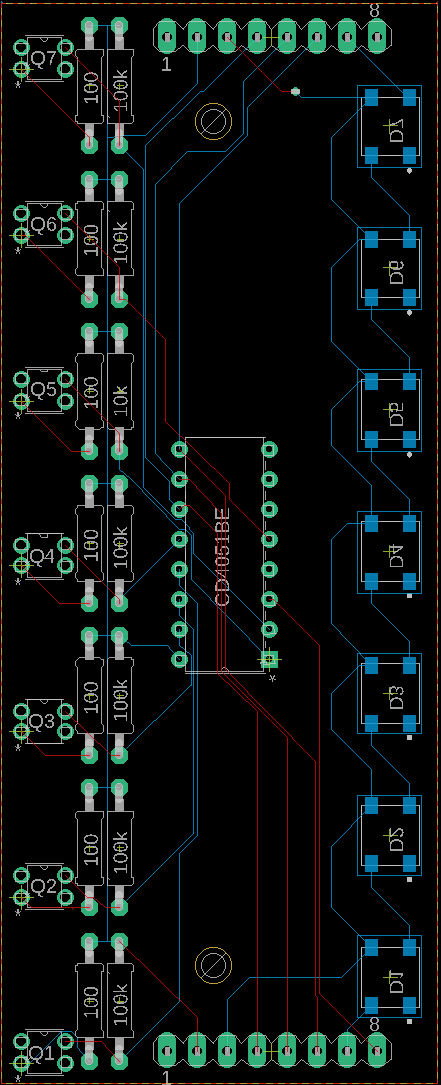
\includegraphics[angle=-90,width=\linewidth]{src/images/7-sensor-board-v0.1.0.png} 
  \caption{} 
  \Description{} 
  \label{fig:7-sensor-board}
\end{figure}

\subsection{Sensor board}\label{sensor-board}

The 49 optical sensors are divided across 7 PCBs each containing

\begin{itemize}
\item
  x7 QRE1113 optical sensors
\item
  x7 100 $\Omega$ resistors
\item
  x7 10 k$\Omega$ resistors \footnote{a update on the design showed these could be reduced to a single resistor.}
\item
  x1 CD4051BE Multipexer
\end{itemize}

A number of sensors were tried before the final system was decided upon. 
Sensors tested for the design included, a 6-degrees-of-freedom inertial measurement unit, reed and hall sensors paired with magnets, and light-dependant resistors mounted to the jack rail.
None of the above satisfied the sensor criteria described and were thus discounted.

Following from the work in \cite{McPherson2013, McPherson2019}, we tested
a system using the Fairchild QRE1113 \footnote{Fairchild, now ON Semiconductor, QRE1113 datasheet \url{https://www.onsemi.com/download/data-sheet/pdf/qre1113-d.pdf}}. The
QRE1113 is a combination infrared LED and phototransistor sensitive to
IR light. The phototransistor of QRE1113 provides data on how much light
is present and in particular how much light is being reflected from a
surface. Since reflected light will be proportional to the distance of
a surface it is a good, close-proximity, distance sensor. Distance is
the way in which the instruments in \cite{McPherson2013, McPherson2019}
function as well the Moog Piano Bar from which it took inspiration.

The limitation for taking a distance approach is that there is not one
but 2 jacks per key. For each jack to be measured independently the data
would need to come from the jacks themselves.

% They \emph{could} be used and individual trigger points set in
% calibration, but this creates new problems.

\begin{figure}  
  \centering
  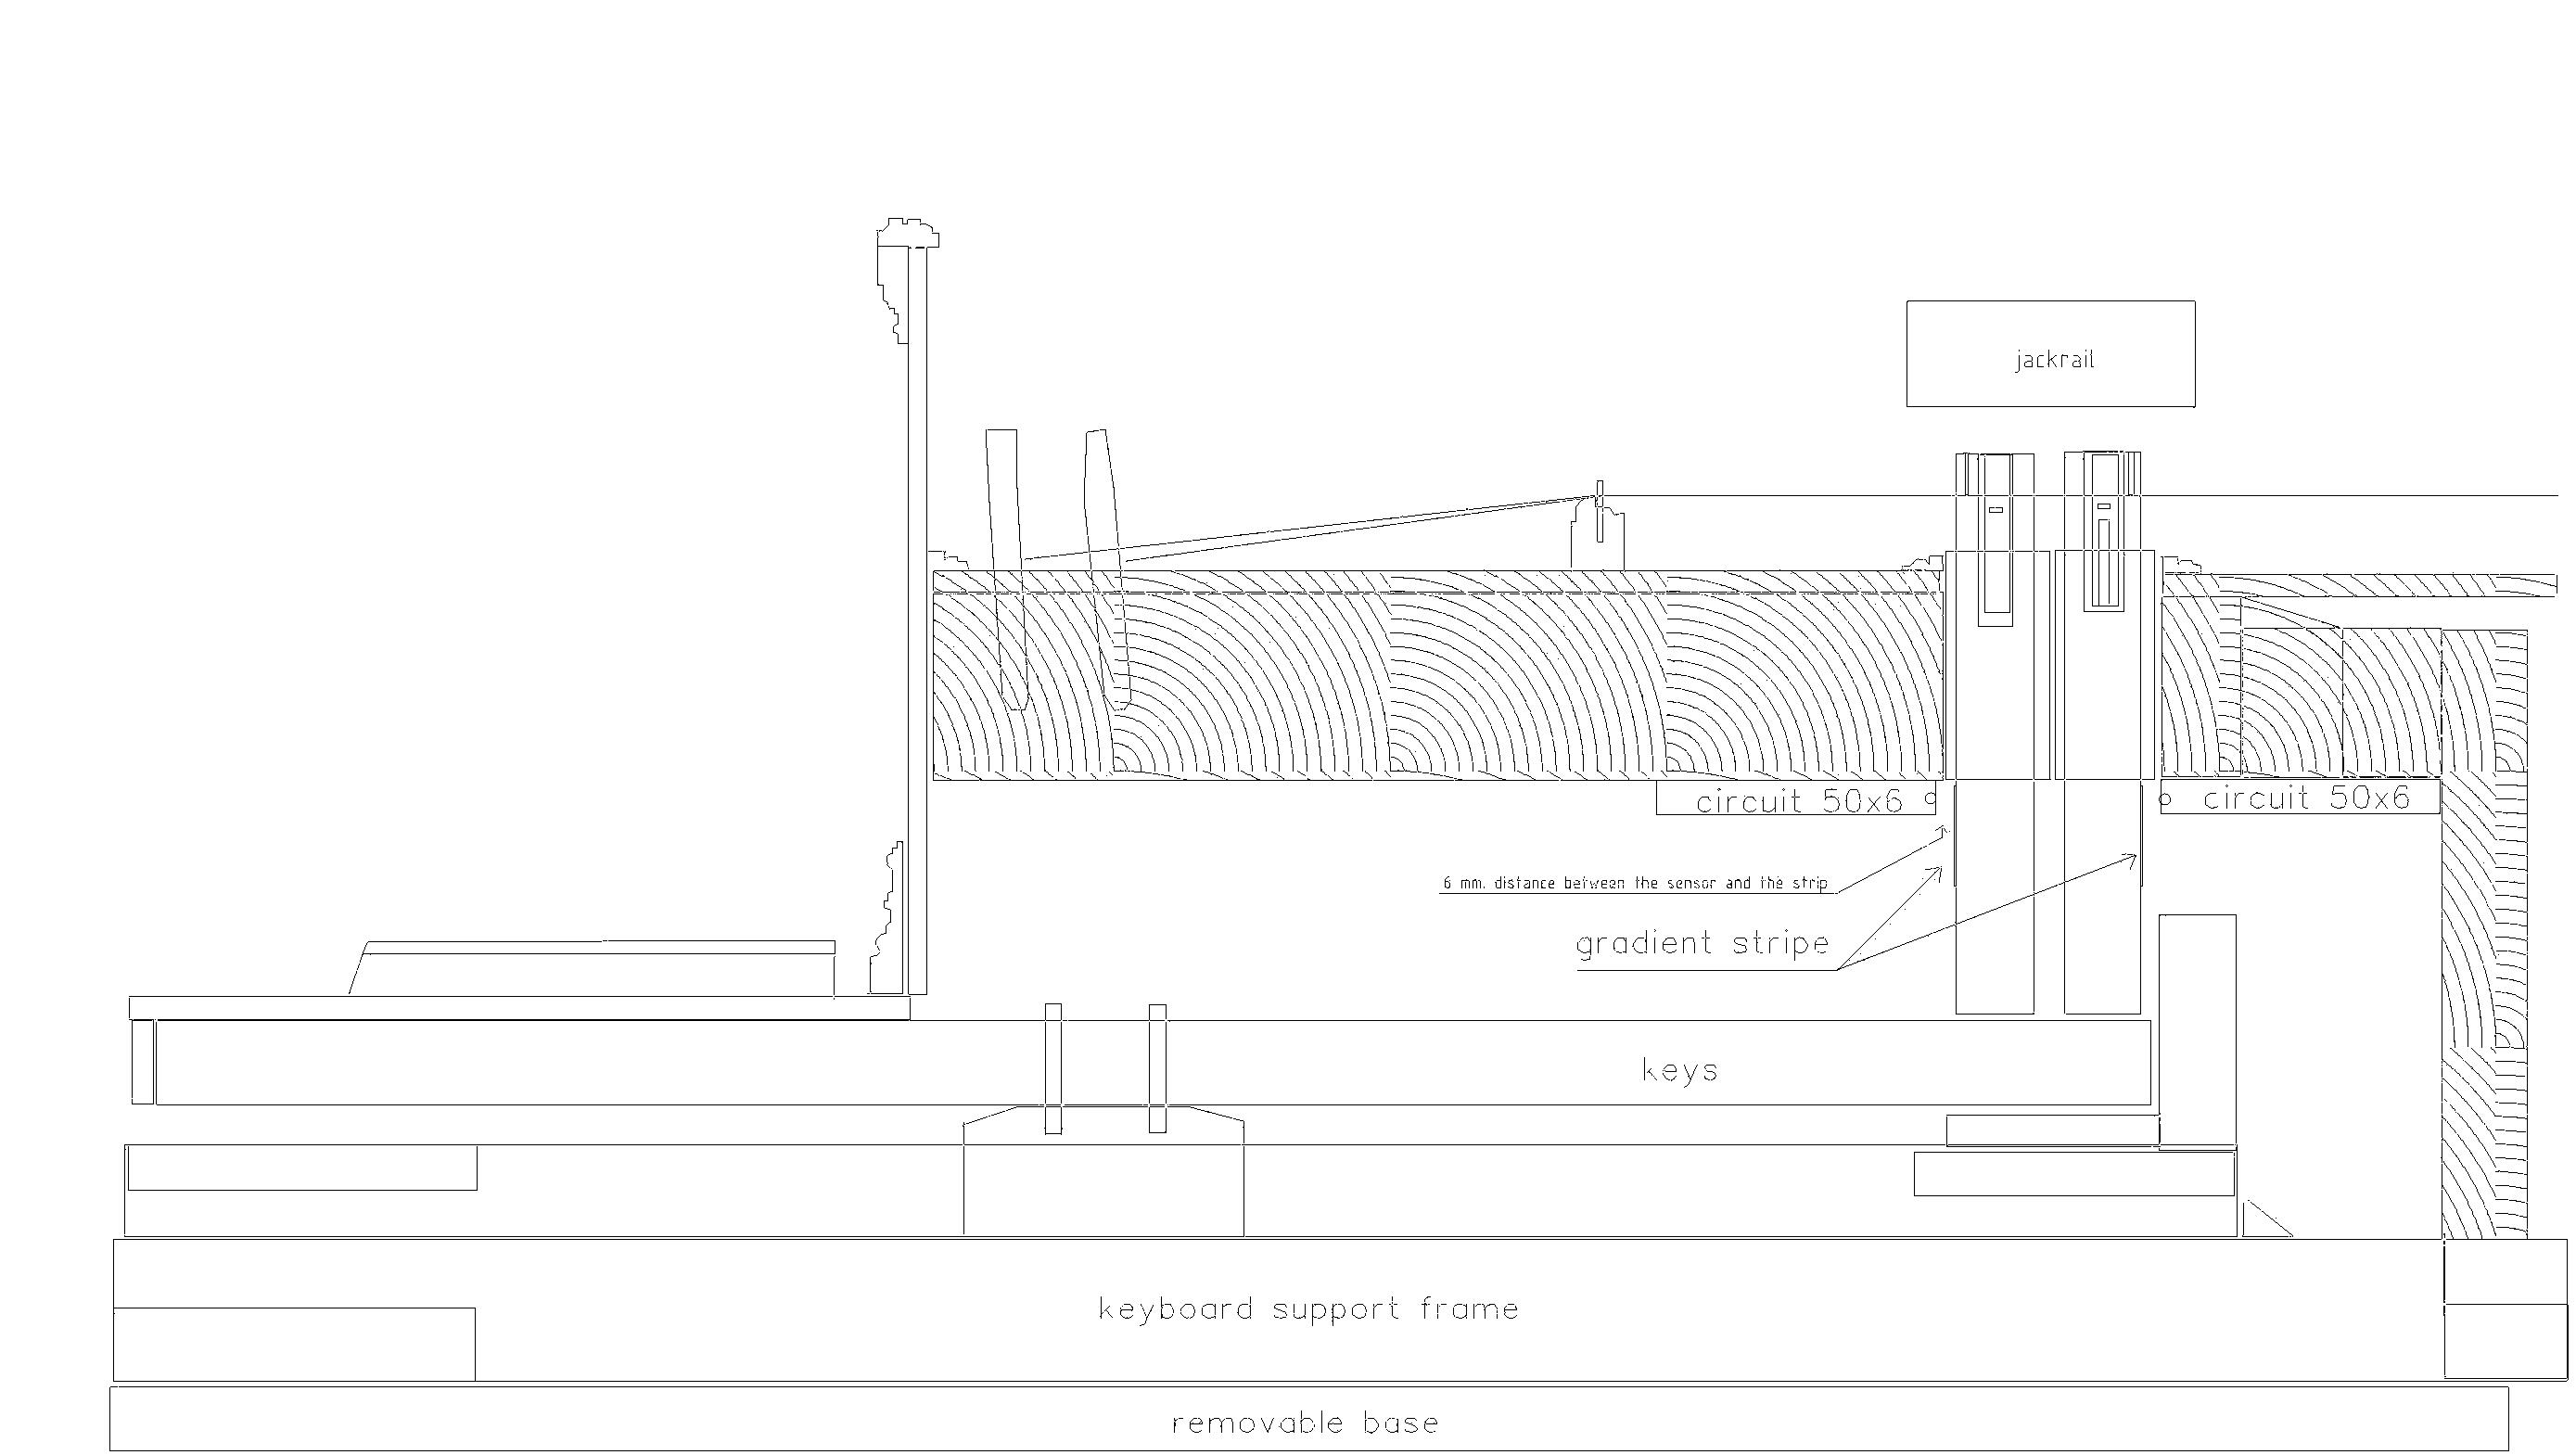
\includegraphics[,width=\linewidth]{src/images/CrossSectionSensorPlacement.jpg} 
  \caption{} 
  \Description{} 
  \label{fig:cross-section}
\end{figure}

Another common application of the QRE1113 is within line following
robots, where an array of QRE1113s are used in conjunction with black
tape or reflective. A motorised system can then use this data to follow the line of tape and adjust its position.

Applied to the jacks was a greyscale gradient printed the length full
travel range of the jack.

For the first iteration this was performed on an inkjet printer and
double-sided tape. For the final iteration the stickers were printed on
(Coala, 1D 100 Gloss P, gloss, white, permanent adhesive, 300g/m2, 100
µm, 1370mm x 50.00m, Solvent/Latex/UV) using a HP Latex 115 and then
cutout with a Summa 150 roll cutter. The printer and roll cutter greatly
reduced the manual labour for cutting stickers meaning the process would
scale from the 3-key to the 49-key model.

% An initial sticker design was used that contained only the gradient. It
% was found that the jacks were sticking in their slots and the edges on the
% stickers easily peeled around the printing The sticker was redesigned to
% be the full length of the jack which avoided the problem of peeling. The
% larger are also mean the stickers adhered better to the jack Some
% trimming was still required of each sticker to avoid them adding extra
% resistance to the jack's movement.

During testing it was found that their was a considerable amount
cross-talk between adjacent sensors. This meant the reading from key
would be affected by the movement of the key next to it. The cross-talk
was assumed to be as a result of light reflecting from other jacks.
Given that IR is used this was difficult to confirm by sight. A set of
baffles was designed for the PCB that would wrap round the jack and stop
light from other jacks or sensors. The baffles were printed on a BAMBU X1 3D
printers using PLA plastic. A dark pigmented PLA was used to avoid IR
light simply being diffused. After the baffles were fitted, the
cross-talk was eliminated.


\subsubsection{RGB LEDs}\label{rgb-leds}

for problems of scale:

Addressing the problem of scale of identifying which key's threshold is
currently being edited.

The LEDs also allowed for easy identification for keys that were outside
of expected values and when a key was triggered. This allowed for visual
identification of malfunctioning or un-calibrated keys.

The LEDs are on the same PCB as the sensors and are hidden when the
name board is in place.2024

Would suggest that this is a necessity of this kind to provide a means
to identify and diagnose LEDs with state.

TLC5940 or other PWM driver such as in \cite{McPherson2013} added
complexity to assembling, but were avoid in favour of Addressable LEDs
with integrated driver. The integrated LEDs share the same data line
which has the limitation where a faulty LED will stop all following LEDs
from working. An individual PWM driver per PCB would allow avoid
situations where failure cascades, but would add complexity in assembly
as the parts are typically SMD. Also, given the LEDs are fixed to the
board and could not be repaired in situ, the solution would be to
replace the PCB regardless of which approach was taken. Given the LEDs
were only used in debugging and calibration and otherwise would not be
visible, a simpler design approach was taken.

\subsubsection{Multiplexing}\label{multiplexing}


The BLE Nano has 8 ADC pins connected to one ADC channel via a multiplexer. 
We avoided the complexity of communicating multiple microcontrollers and instead used a Texas Instruments CD4051B multiplexer on each sensor board.
An 8-channel multiplexer was chosen as the model has 49-keys and a division of 7 PCBs each containing 7 sensors.
The multiplexer reduced the 7 sensor signals to a single channel. The CD4051B is addressed with a 3-bit which necessitates 3 digital channels.
Transistor / Op-amp circuit could have been used similar to the one in
\cite{McPherson2013}. Given time constraints it was beneficial to continue using and entirely THT based designed for easy assembly.

% \subsection{PCB design}\label{pcb-design}

% EAGLE PCBs designed using EAGLE. 

% Worth noting that AutoCAD has
% deprecated EAGLE and the programme will no longer be supported from
% 2026 Project files will need to be transitioned to another standard,
% likely the KiCAD programme.

% trade off between limiting number of boards required and allowing
% compensation for variation in pitch.

% Smaller PCBs means that spacing could be adjusted to accomodate the
% changes in pitch between jacks. It also allowed for a modular approach
% where any PCB could swapped for minimal cost.


% \begin{itemize}
% \item
%   x7 QRE1113
% \item
%   x7 100R
% \item
%   x7 10kR
% \item
%   x1 CD4051BE Multipexer
% \item
%   jack / sensor pitch by board
% \item
%   7 boards adjust for pitch/spacing error
% \item
%   modular, replaceable
% \item
%   orientation problems

%   \begin{itemize}
%   \item
%     legs break easily
%   \item
%     end mount like A.P.Mc. time consuming
%   \item
%     problem

%     \begin{itemize}
%     \item
%       milling out keys
%     \end{itemize}
%   \end{itemize}
% \item
%   designed from distance
% \item
%   striped lines across pcbs
% \item
%   problems

%   \begin{itemize}
%   \item
%     additional terminals uneeded resulted in lots of additional work
%   \item
%     long cabling increase risk of breaking
%   \end{itemize}
% \item
%   solutions

%   \begin{itemize}
%   \item
%     striping all ADC lines with FFC
%   \item
%     solder pads to select channel
%   \end{itemize}
% \end{itemize}



\subsection{Controller Board}\label{controller-board}

Controller board designed around Arduino nano form factor. The Nano is
connected through headers to allow easy switching between chips. Should
another chip in a Nano for factor be found it could supplant the current
Nano without any need for a redesign.

The first version of the board exclusively used 2.54mm pitch headers.
The reasons for this were flexibility when creating cable looms and to
leave open the possibility of rewiring the PCB.

This was the case for the LEDs as they initially were to be powered on
5V. It was discovered that the 3v regulator of the nano was sufficient
to power all LEDs at a lower brightness while reducing current draw.
Since brightness was not important.

The 2.54mm pitch headers had two major drawbacks. First, the orientation
of the cables could be reversed, which in the best case scenario would
simply mean the system did not work correctly and in the worst case it
could potentially damage the components.

Secondly, the headers do not connect securely and wait of the cabling
was enough for components to become disconnected as the harpsichord was
handled.

To address this, once the wiring for the controller board was finalised
a new design was drafted this time using JST-PH connectors. No
commercial cables were immediately available in the configuration and
length required, as such a cable loom needed to be made which meant
crimping cables by hand. A crimping tool from JST is prohibitively
expensive compared to the cost of other components in the project
\footnote{from RS \url{https://uk.rs-online.com/web/p/crimp-tools/6880877}
£508 (inc. VAT)}. The crimping tool also appeared to be uncommon and was
not readily available in the workshops at the project's disposal.
Eventually a tool was found, but an alternative approach was also
researched in order to maintain the criteria of accessibility.

A locator was adapted from a creative commons STL model
\footnote{\url{https://www.thingiverse.com/thing:1646016}} that allowed a
generic crimping tool to be adapted for use with JST-PH crimps. 
The locator was printed using a Bambu X1 3D printer. 
A second alternative was assembling cables from other sets that were at hand.

\subsubsection{Arduino Nano BLE}\label{arduino-nano-ble}

Arduino Nano BLE was chosen for a few reasons. The Nano form factor was
appealing as it would allow for easy changes between chipsets without
requiring any rewiring and thus no new PCBs would need to be created if
a better alternative was found later in the project. Another benefit to
the Arduino Nano boards was that typically had native-USB meaning the
could be programmed as a hardware USB MIDI device directly.

The Nano BLE was used in the initial stages for its integrated inertial measurment unit.

When it was finalised that the project would proceed using the QRE1113 a
number of microcontroller units (MCU) were considered.

The MCUs considered were the Arduino Nano 33 IoT, Arduino Nano 33 BLE,
Arduino Nano ESP32 and STM32 NUCLEO-L031K6.

A rough performance test was later carried out using an STM32
NUCLEO-L031K6, a Nano ESP32 and the BLE. The Nano BLE was found to be
more performative. To execute a single sensor read cycle of the firmware
the STM32 took 40ms, and both the Nano ESP32 and Nano BLE required 11ms
on average. The Nano ESP32 had high variability so it was decided to
continue with the Nano BLE. 

% Further discussion of using ESP32 continues
% in \textbackslash section\{Going forward\}

BLE functionality also meant if the cable connection between the nano
and computer running audio synthesis was impractical, BLE MIDI was
available as a fallback. The Nano BLE also has a 12-bit DAC, which
provided a contingency should the default 10-bit not be sensitive enough
for the signal from the sensors.

Initially a Nano IoT was used for both WiFi and Bluetooth Low Energy
functionality, but it was found that 2 ADC channels were in fact not
useable and would have required additional multiplexers.

\subsubsection{EEPROM / NVRAM / FRAM}\label{eeprom-nvram-fram}

There would need to be the ability to store values on non-volatile
memory so that the electronics could be powered-down without losing
data.

Adjusting the values through firmware would not have been flexible or
practical. Instead an Ferroelectric RAM unit was chosen and connected
using an SPI interface. NVRAM or EEPROM would have sufficed and the FRAM
was primarily chosen for it's ready availability.

Most microcontrollers have some variety of non-volatile program memory
that can be read and writ accessed but in most cases this memory is
cleared during compilation and re-flashing. The small cost was far
outweighed by the potential for data loss if using onboard RAM.

% \emph{It is worth noting that the FRAM model chosen stopped being
% available during the project, meaning any future iteration would need to
% adjust for another board in firmware}

% The firmware was structured in a way that the interface could be changed
% so long as the code required for any other board would comply with
% function arguments and outputs. 

% Worth noting the fragility and
% volatility when designing this kind of project and how easily it is for
% the project to become broken.

SD card would provide an easier way to interact with calibration data.
The position of the controller board did not permit easy access.
reliability and speed was preferred over storage capacity.


\subsection{3D printing}\label{d-printing}

Access to a 3D printer is was vital to the success of the project. Given
the proliferation of 3D printing, particular in maker spaces in
universities it was deemed an unreasonable requirement. 3D printed parts
include the support brackets for PCBs, the baffles for the sensors,
locator for crimping JST-PH crimps and a mount for the MacMini used for
audio synthesis.

The printer used throughout the project was a Bambu X1-Carbon using
recycled PLA filament.

Support brackets and baffles were made for the project while the MacMini
bracket and JST locator were sourced from creative commons models.

Any colour of filament can be used, though it is advised to use a dark
coloured filament for the baffles.

See each corresponding section for more detail on 3D printed components.

\subsection{Power}\label{power}

All electronics draws around 1.1amps of current at 5V with some
fluctuation during boot.

Arduino BLE has some functionality disabled to limit current draw.

Ideally the unit could be bus powered from USB.

The sensors are in a state of constantly drawing power. It is possible
that powering only when data is required could be reduce power enough.

Current designs have a separate MIDI device for each jack row. Combining
the devices and also reducing current draw to below the common 0.5 amps
for a USB port would certainly be a challenge.

\section{Firmware Design}\label{firmware-design}

Arduino platform chosen for wide adoption, relative ease of use and
library support for components.

Firmware checks components are connected then reads the FRAM to see if
threshold data is already present. The rotary encoder and it's momentary
switch are polled for any change in state. A key is selected with the
rotary encoder while the momentary switch is used for changing between
states for key selection and threshold adjustment A double click of the
rotary encoder writes the current threshold values to FRAM. The sensors
for the current multiplexer channels are polled. If any sensor reads
above the threshold when it was previously below a MIDI On message is
sent. For the reverse case where the value was below the threshold when
it was previously above, a MIDI Note Off message is sent.

% \subsection{Project structure}\label{project-structure}

% The project is separated into three repositories encapsulating

% \begin{itemize}
% \item
%   Firmware
% \item
%   Keyboard CAD Data
% \item
%   PCB CAD Data
% \end{itemize}
% 
% \subsubsection{Firmware}\label{firmware}

% Firmware repository contains all firmware for the full and smaller
% models and components.

% \subsubsection{Keyboard}\label{keyboard-1}

% The Keyboard repository contains all plans for fabricating the keyboard,
% measurements and 3D models of the jacks.

% \subsubsection{PCB}\label{pcb}

% PCB repository contains the EAGLE files for creating the sensor and
% controller boards.

% Given the regular spacing of components, scripts for automatic placement
% of components based on parameter of jack pitch spacing and number of
% sensors per jack.

\section{Implementation}\label{implementation}

\begin{figure}  
  \centering
  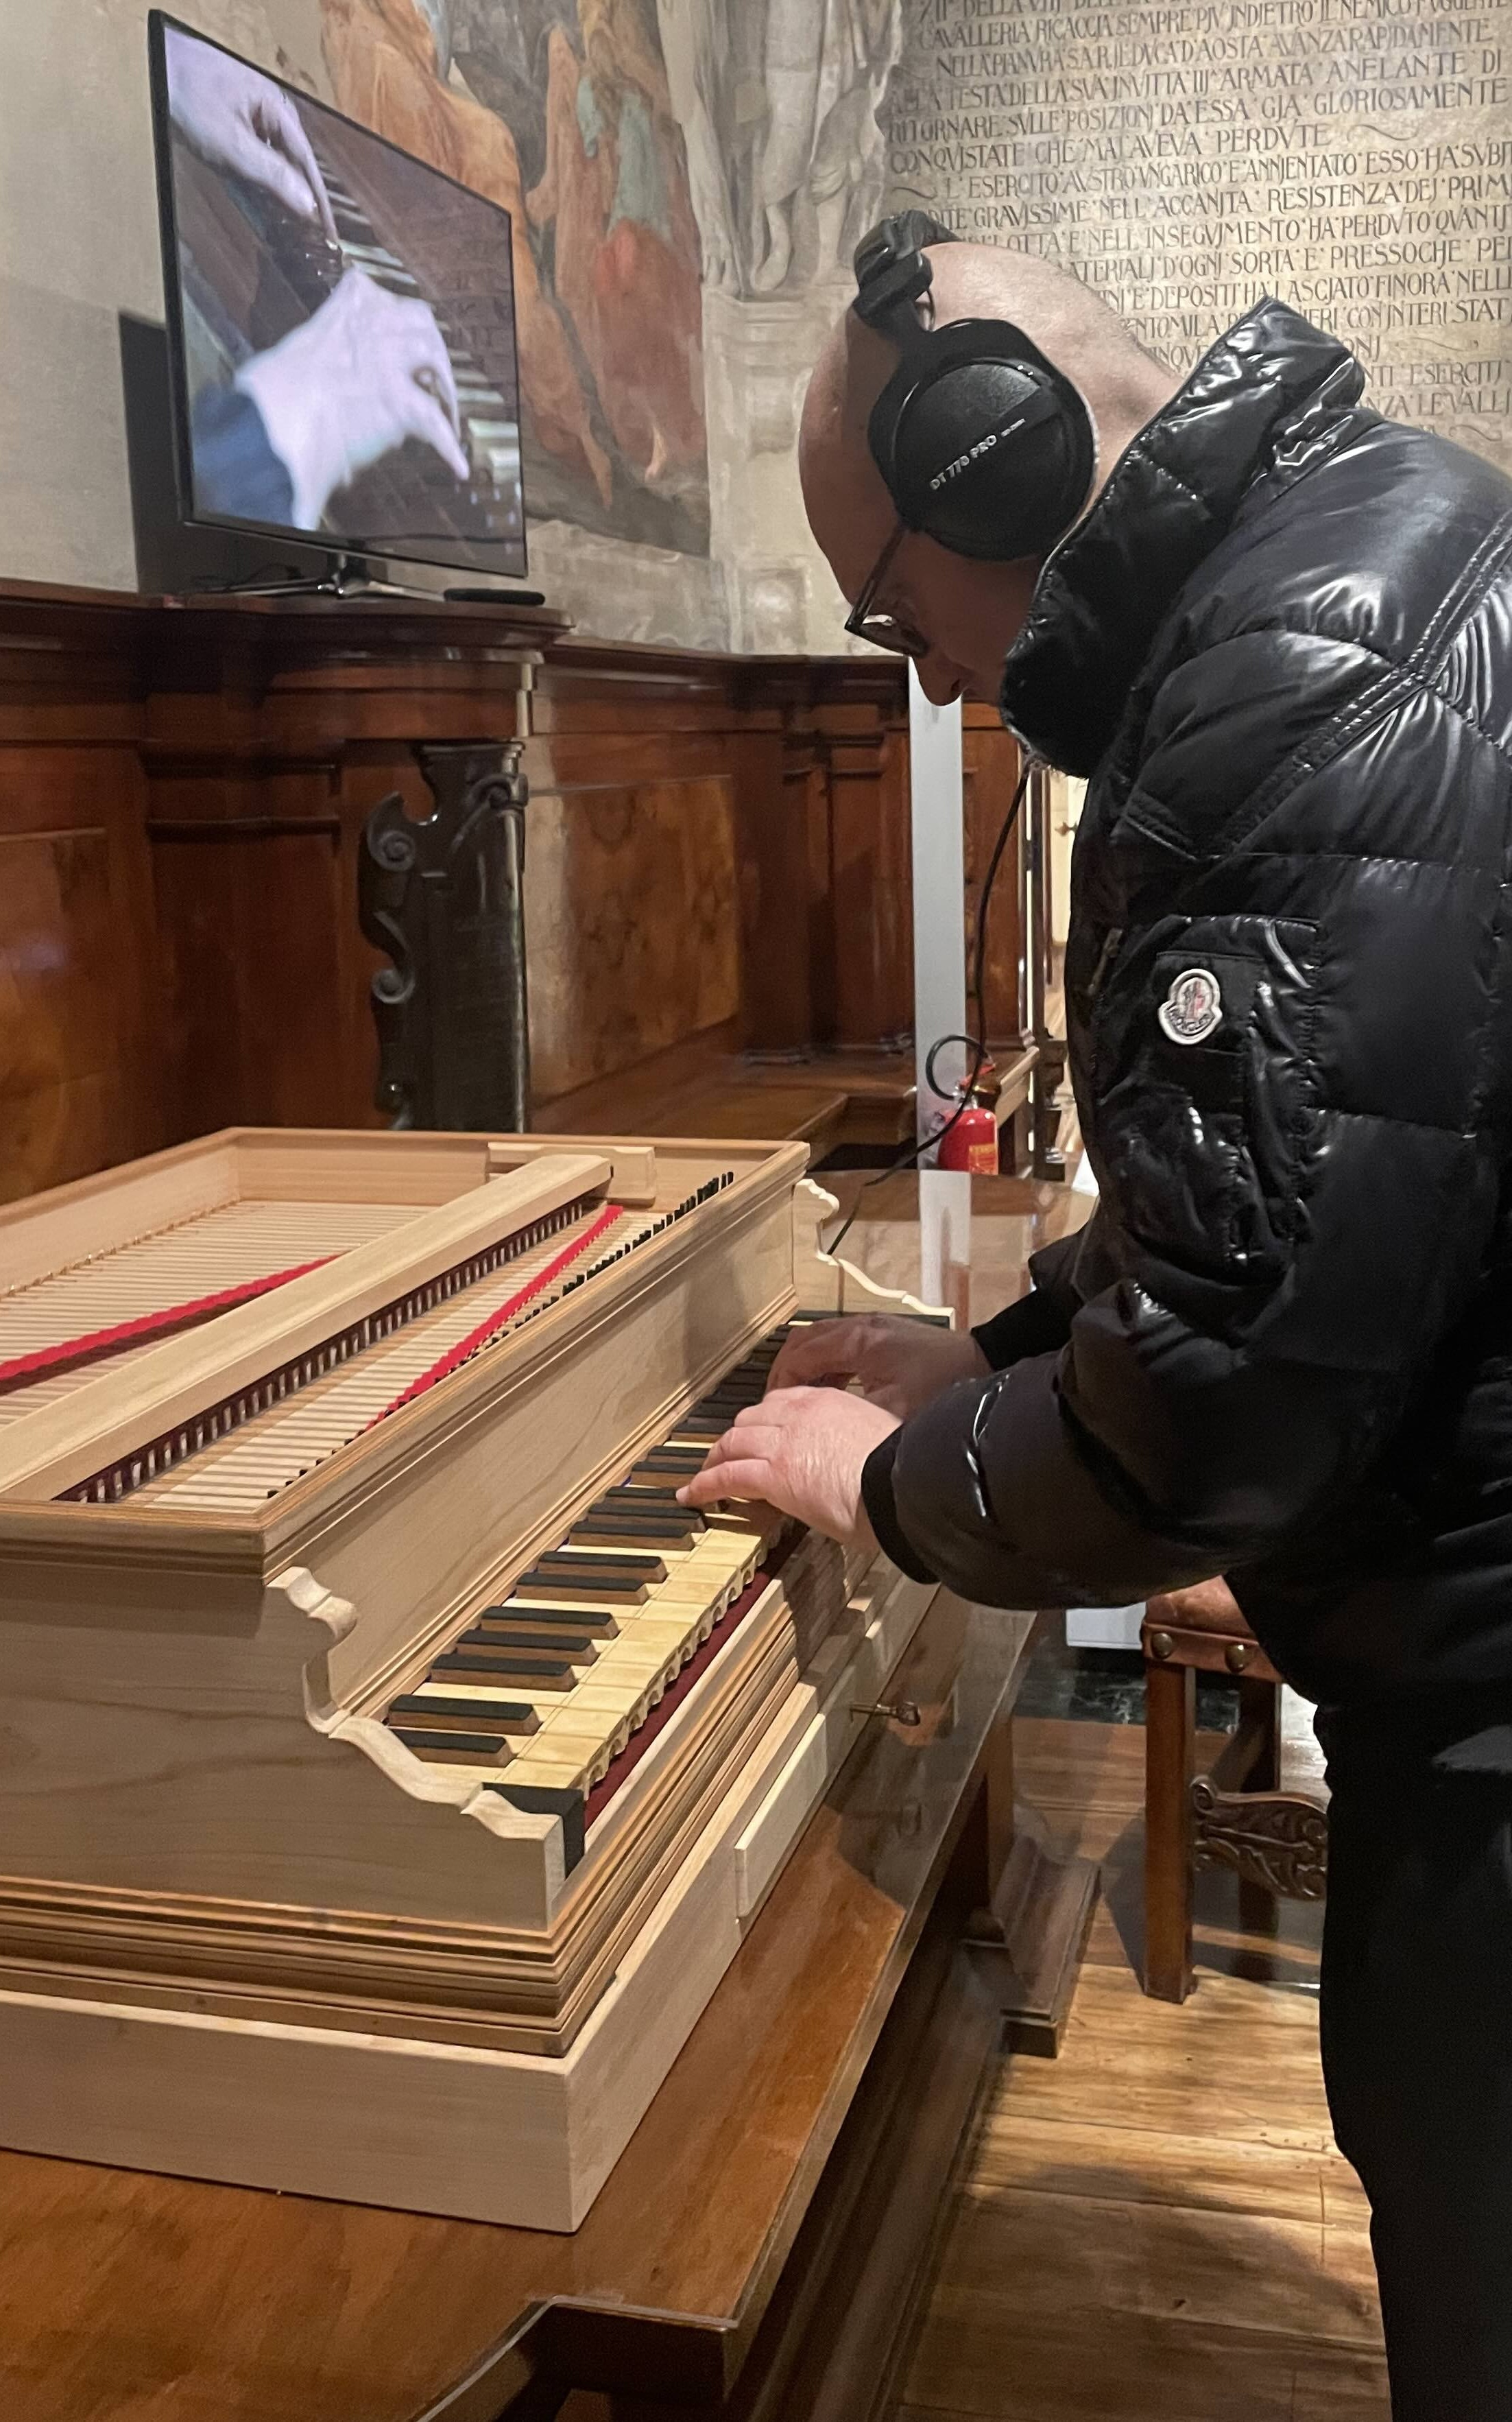
\includegraphics[,width=\linewidth]{src/images/exhibition-user-1.jpeg} 
  \caption{} 
  \Description{} 
  \label{fig:exhibition}
\end{figure}

\subsection{Installation}\label{installation}

The electronic components were partly pre-assembled at the university of
Edinburgh. Though all measurements were known ahead, enough flexibility
was needed to allow for problems to solved in situ.

The final assembly took place at the NEMUS lab at the University of
Bologna over the final week in October 2024 for delivery at San
Colombano for exhibition in the first week of November in 2024.

A misreading in the original clearance between the keys and the PCB
meant that the keys were blocked entirely from moving. A 10mm by 15mm
section was milled out of each key to create extra
clearance. The milling required the removal, shortening and refitting of
the leather pads for the jacks. The extra work
added an extra day to the full install.

\begin{figure}  
  \centering
  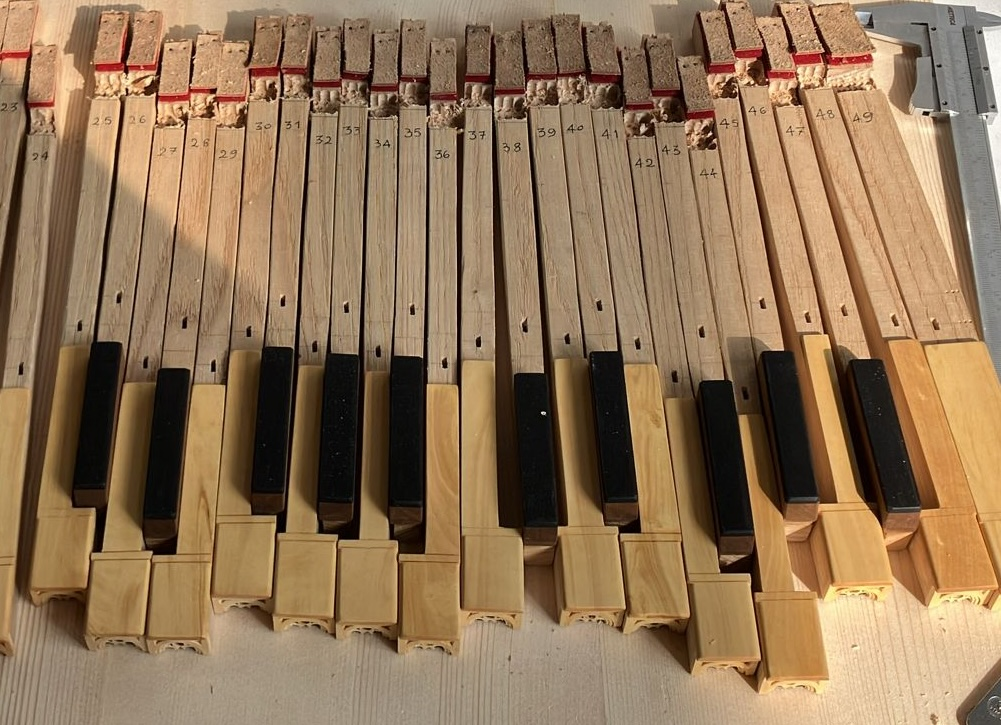
\includegraphics[width=\linewidth]{src/images/keys-milled.jpeg} 
  \caption{} 
  \Description{} 
  \label{fig:milling}
\end{figure}

A redesign of the PCBs meant that removing the material would no longer
be necessary.

The PCBs shared power and data lines for components with the exception
of the output from the multiplexer. Ribbon cable was cut to size to
allow for some room to readjust the distance of the sensors from the
jacks. The data signals from each PCB were connected using a separate
cable loom. Soldering cables and inspecting each join required another
day work. This did allow for readjustments to the position of the
controller board Measurements of the rear chamber did not match with the
Mac Mini that was to be used a different layout was decided for fitting
the controller board/ Cutting cables to size allowed for a great deal of
flexibility but at the cost of time. After the first install it was
clearer what constraints were in place for fitting and an alternative
wiring system using flat flex cable was implement (discussed in
\textbackslash section)

Fitting PCBs required the removal of all keys. The support brackets were
assembled and screwed into the the underside. With the harpsichord on
it's back the sensors were tested to ensure an expected range.
Self-tapping round head screws were used to to attach the brackets. The
screws were not over tightened to allow for brackets to move. The
brackets were not easily adjusted once the key were replaced. Adjusted
to a best average with subsequent adjustment carried out on the
microcontroller.

As the PCBs were fitted the jacks had the gradient stickers applied to
them. The jacks had been coated with a varnish on the short side to
provide a better surface for the stickers to adhere to. After the
stickers were applied excess material was trimmed from each jack. The
jack were then check that they moved freely in their slot.

After fitting the PCBs preliminary calibration was carried out. Before
the keys were refitted the jacks were put back in place. The data from
each key was confirmed to be in a similar range. Any key showing
anomalous data had it's jack removed and re-inspected. The PCB fitting
process and refitting required another day as faults were found in
wiring or misalignment of the stickers. After the sensors were
confirmed to be functioning the keys were put back.

The calibration workflow was with \anon{Dr. Craig Webb} who was unfamiliar with
the system. Adjustments were made to the firmware to to make it more
intuitive for the user. Addressable LEDs became vital as it allowed for
easy identification of the key being calibrated. They were also used to
identify any keys whose current reading was beyond what was expected.

The rotary encoder was used as the interface to select a key, adjust
it's threshold and update the Ferroelectric RAM (FRAM) with new values.

A process was implemented where the key was selected by playing, but
this caused problems in situations where the data was unusual due to
misalignment of the sensors.

This would likely be a better system for when the keyboard was fully
operational.

\begin{figure}  
  \centering
  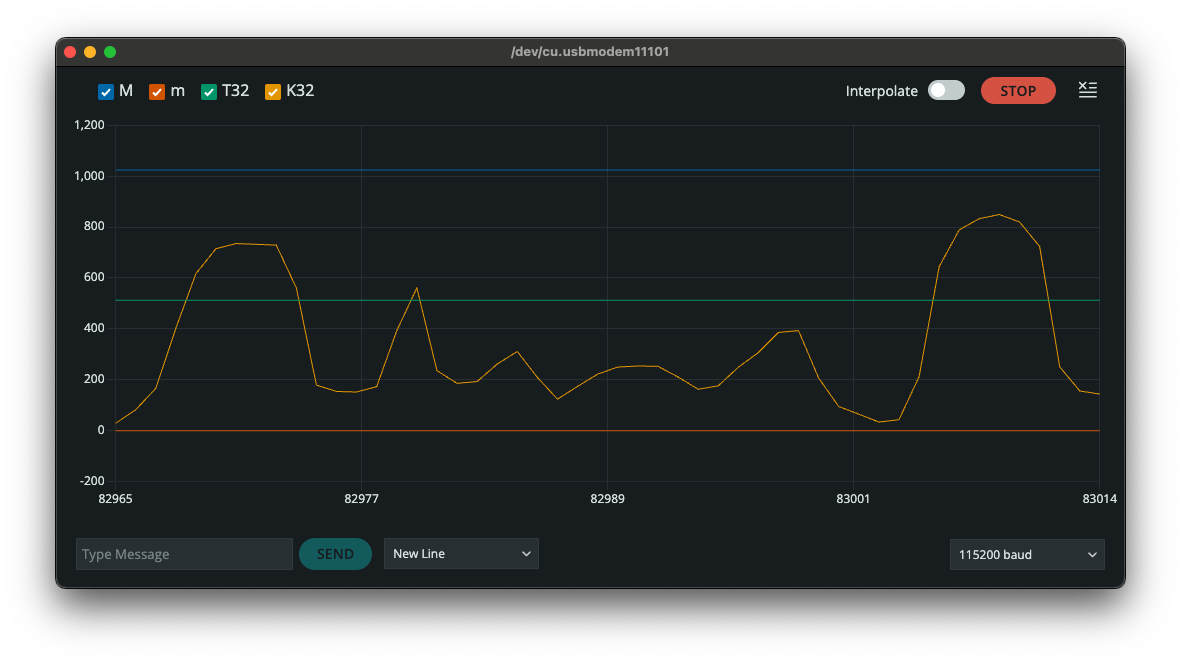
\includegraphics[width=\linewidth]{images/serial_monitor.png} 
  \caption{} 
  \Description{} 
  \label{fig:serial_monitor}
\end{figure}

The thresholds were calibrated visually utilising the serial plotter of
the Arduino IDE (Figure \ref{fig:serial_monitor}) and the open source MIDI
Monitor software \footnote{\url{https://github.com/krevis/MIDIApps}}.

\begin{itemize}
\item
  partial pre-assembly
\item
  handsolder components

  \begin{itemize}
  \item
    analog lines
  \end{itemize}
\item
  connecting supports
\end{itemize}

\subsection{Context}\label{context}

Designed as part of an exhibition for the museum San Colombano in
Bologna. Instruments is to be played by general public as a means of
interacting with items in the collection that are no longer in playing
condition. Audience of one who listens via headphones.

The strings of the interface are damped with felt strips. The damping
did change the tension and thereforew the feel of the strings so
adjustments needed to be made to the tuning to accomodate for this.

\begin{itemize}
\item
  in museum context
\item
  strings damped
\item
  headphones
\item
  interfacing with kontakt spitfire library
\item
  display

  \begin{itemize}
  \item
    secure storage and access
  \item
    interface to the public
  \end{itemize}
\end{itemize}

\subsection{Calibration}\label{calibration}

Finer calibration carried out with the guidance of \anon{Catalina Vincens} as
an expert harpsichord performer

\begin{itemize}
\item
  sensor surface

  \begin{itemize}
  \item
    printed gradient
  \end{itemize}
\end{itemize}

\section{Conclusion}\label{conclusion}

\begin{itemize}
\item
  scale
\item
  time scale
\item
  working at distance
\item
  limitations

  \begin{itemize}
  \item
    latency
  \item
    deprecation

    \begin{itemize}
    \item
      software

      \begin{itemize}
      \item
        EAGLE
      \end{itemize}
    \item
      hardware

      \begin{itemize}
      \item
        FRAM
      \end{itemize}
    \end{itemize}
  \end{itemize}
\end{itemize}

\section{Going forward}\label{going-forward}

\begin{itemize}
\item
  Velocity, aftertouch
\item
  second jack row
\item
  reducing latency
\item
  alternative sensor surfaces
\end{itemize}

A limitation in the design is the variability in positioning of tag,
especially when they need to be reapplied. A jig was designed for
applying tags, but could not be printed in time for installation. Even
with a jig, some tags had to be readjusted by hand regardless. Long term
this has implications on how to maintain the interface.

Taken a different approach to what surface is used. Preliminary test
were taken using Laser Cutting and CNC to fabricate Jack bodies. Laser
cutting results in a loss of material that has too much variability. The
edge of the jack body will be charred. The material also needs to be
reliable. on the advice of two luthiers, \anon{Roberto Livi} and \anon{Jonathan Santa
Maria Bouquet} at \anon{Edinburgh}, Plywood and MDF have problems with
variations in humidity, tear-out and delamination.

Some tests were carried out using a notched jack body that was 3D
printed. The notch means that as the jack raises, the forward material
acts like a shutter. No reasons that this could not be CNC though a
variety of materials would be needed. Traditional material used is xx
though need to test of the material is naturally reflective enough or if
a coating would need to be applied.

Outputs of the NEMUS project will also include numerically simulated
non-linear plucked string models with which the device can interact. A
bespoke sound synthesis engine to leverage data from both jack rows
which will also be open-sourced. Design for instrument to be compatible
with standard MIDI instruments as well software designed for the full
data output.

A second interface designed more closely to the Trasuntino style
instrument commissioned by the \anon{NEMUS} project with \anon{Roberto Livi}. Using
lessons learned for the first iteration the second can make better
accommodations for internal electronics. Interface to be used for a
performer study and used for performance with a numerically simulated
sound synthesis engine.

Testing current sensors in conjunction with force sensitive resistors to
research if a impulse response for the pluck can be extrapolated.

Future novel designs for an interface that would utilise velocity and
aftertouch messages in software. This would be applicable for numerical
simulations of strings. A bespoke piece of software would also allow
for direct mapping of jack rows to registers. There is enough data to
implement functionality for velocity and aftertouch MIDI messages and
simply needs to be activated in the firmware. (Hyperinstruments
\cite{nime2024_20})

seat vibrations \cite{MusicalHaptics2018_07}

\begin{itemize}
\item
  ``there is a general connection between vibrations and the perceived
  quality of music reproduction''
\item
  ``influence of vibrations on loudness perception at low frequencies''
  Evaluation
\end{itemize}

\subsection{improvements}\label{improvements}

\begin{itemize}
\item
  ESP-IDF

  \begin{itemize}
  \item
    latency half
  \item
    workload high
  \end{itemize}
\end{itemize}

A current limitation is the latency in triggering MIDI output. Currently
the latency is around 20 ms, but should ideally be closer to 5ms.

An obvious approach would be merely changing the microcontroller. A test
was carried out using an Arduino Nano ESP32 which is a NORA-W106, a
module with a ESP32-S3. The benefit of this microcontroller is that it
would allow simply the board to be swapped and the rest of the PCB
designs would be unaffected.

Using the Espressif development framework ESP-IDF and following the same
logic as the original firmware source, the latency was reduced to around
10ms. ESP-IDF allows access to functionality of the ESP32 that is not
exposed in the Arduino libraries. It is possible that the 10ms latency
could be improved upon, but there would be a cost in the form of
development time. Consideration would need to be made on how to port
existing code or whether to completely re-write the firmware.

\begin{itemize}
\item
  avoid soldering cabling
\item
  power indicators on pcbs

  \begin{itemize}
  \item
    debug if problem is power related Add power small power LEDs to the
    each PCB. It was not common for a board to not be functioning and
    thye result to be that the power was not correctly connected.
    Especially when the power is connected via something such as an FFC
    cable where it is easy to plug-in the wrong way especially when
    fitting is to be carried out by someone unfamiliar with the system.
    Power LEDs would quickly confirm whether the problem was power
    related. They would have to be small enough and low enough current
    draw to avoid glare or being mistaken with other indicator LEDs To
    continue using THT components, the choice would have to be made
    carefully.
  \end{itemize}
\end{itemize}

\section{Ethical Standards}\label{ethical-standards}

To ensure objectivity and transparency in research and to ensure that
accepted principles of ethical and professional conduct have been
followed, authors must include a section ``Ethical Standards'' before
the References. This section should include (if relevant): information
regarding sources of funding, potential conflicts of interest (financial
or non-financial), informed consent if the research involved human
participants, statement on welfare of animals if the research involved
animals or any other information or context that helps ethically situate
your research. For help with the ethics section, feel free to ask on the
NIME forum: \url{https://forum.nime.org}.
